\chapter{Optics}
	\index{Optics} Optics is the study of light and how that light interacts with matter.  There are two general fields of Optics: \textit{Geometric Optics} and \textit{Physical Optics}. Geometric optics studies how rays of light travel, while physical optics studies how multiple rays of light interact as waves.  
	
	An important constant in the field of optics is the speed of light.  The speed of light in empty space is exactly:	\index{Speed of Light}
	\begin{mdframed}[backgroundcolor=green!20!white]
		\begin{equation*}
		c = \SI{299792458}{m/s}
		\label{equation:speedoflight}
		\end{equation*}
	\end{mdframed}	
	
	The symbol used is \textit{c} because the speed of light is constant in all frames of reference.  This fact will be discussed in more detail in \color{red} (Insert REFERENCE  HERE.) \color{black} You will often see this number rounded to $2.998 \times 10^8$ m/s or even $3.0 \times 10^8 $m/s.
	
	
	
	
	\section{Geometric Optics} \index{Geometric Optics}
	
	While light in empty space always travels at the same speed, $c$, light can be slowed down when it travels through a medium.  This leads to some phenomena that we may encounter in everyday life.  
	

	\subsection{Refraction} \index{Refraction}
		
	\textit{Refraction} is a phenomenon associated with how light changes direction as it moves from one medium to another, due to the change in the speed that light travels at in each of the media.  This is often demonstrated by looking at a pencil in a glass of water, or a fish in a pond.  
	
	\subsubsection{The Index of Refraction}
	The index of refraction \index{Index of Refraction} is the ratio of the speed of light in a vacuum to the speed of light in a material.  It can be calculated as follows:
	
	
		
	\begin{mdframed}[backgroundcolor=orange!20!white]
		
		\begin{equation}
		n \equiv \frac{c}{v_m}
		\label{equation:indexofrefraction}
		\end{equation}
	\end{mdframed}
 
 where $n$ is the index of refraction, $c$ is the speed of light in empty space, and $v_m$ is the speed of light in the material.  
 
 
 	\begin{mdframed}[backgroundcolor=blue!10!white]
 	\begin{center}	
 		\textbf{Example \thesection.1}	
 	\end{center}
 	
 	\textbf{Problem: } Light travels at a speed of $2.254 \times 10^8$ m/s in water.  What is the index of refraction of water? 
 	
 	\textbf{Solution:} Using the definition of index of refraction, we find:
 	
 	\begin{equation}
			n \equiv \frac{c}{v_m} = \frac{2.997 \times 10^8 \, \si{m/s}}{2.254 \times 10^8 \, \si{m/s}} = 1.330
 	\end{equation}
 \end{mdframed}
 
 You may notice that the index of refraction is unitless, since all units cancel in the calculation.   A list of indices of refraction can be found in Appendix \ref{tab:refraction} on  \cpageref{tab:refraction}.
 
 
	
		\subsubsection{Snell's Law} \index{Snell's Law}
		\textit{Snell's Law}, named for the Dutch physicist Willebrord Snell, explains that light always takes the path of least time between two points.  When light travels in a single medium of constant optical density, it travels in a straight line.  However, when light changes medium, it will change direction.  	
		
		
		There are several components and measurements that should be included on a diagram in this situation.  		
		\begin{itemize}
			 \setlength\itemsep{0em}
			\item The \textit{interface} is the boundary where the two materials meet.  
			\item The \textit{normal} is an imaginary line perpendicular to the surface.  
			\item The \textit{incident ray} is the ray of light that is traveling toward the interface.
			\item The \textit{refracted ray} is the ray of light traveling away from the interface.  
			\item The \textit{incident angle}, $\theta_i$ is the angle between the incident ray and the normal.
			\item The \textit{refracted angle} $\theta_r$ is the angle between the refracted ray and the normal.  			
		\end{itemize}
		
		
		A diagram that shows a ray of light traveling from air into water might look like this:
		\begin{figure}[H]
			

		\begin{center}
			

		\begin{tikzpicture}[thick,scale=0.5, every node/.style={scale=0.5}]
		
		% define coordinates
		\coordinate (O) at (0,0) ;
		\coordinate (A) at (0,4) ;
		\coordinate (B) at (0,-4) ;
		
		% media
		\fill[blue!15!,opacity=.3] (-4,0) rectangle (4,4);
		\fill[blue!60!,opacity=.3] (-4,0) rectangle (4,-4);
		\node[right] at (2,2) {Air};
		\node[right] at (2,-2) {Water};
		\node[] at (2,0) {Interface};
	
		
		% axis
		\draw[dash pattern=on5pt off3pt] (A) -- (B) ;

		
		% rays
		\draw[red,ultra thick,reverse directed] (O) -- (130:5.2);
		\draw[red,directed,ultra thick] (O) -- (-70:4.24);
		
		% angles
		\draw (0,1) arc (90:130:1);
		\draw (0,-1.4) arc (270:290:1.4) ;
		\node[] at (280:1.8)  {$\theta_{r}$};
		\node[] at (110:1.4)  {$\theta_{i}$};
		
		\end{tikzpicture}
		\caption{A diagram of light traveling from air into water.}
		\end{center}
		\end{figure}		
		
		In a diagram such as above, it can be seen that the path of least time is given by the following mathematical representation of Snell's Law: 
		
		
			\begin{mdframed}[backgroundcolor=orange!20!white]
			
			\begin{equation}
			n_i \sin(\theta_{i}) = n_r \sin(\theta_{r})
			\label{equation:snellslaw}
			\end{equation}
		\end{mdframed}
	
	
		 	\begin{mdframed}[backgroundcolor=blue!10!white]
			\begin{center}	
				\textbf{Example \thesection.2}	
			\end{center}
			
			\textbf{Problem: } Light travels from water (n=1.33) into diamond (n=2.417).  If the angle of incidence is $45 \degree$, what is the refracted angle?  
			
			\textbf{Solution:} Begin by drawing a (partial) diagram:
			
			\begin{center}
			
			
			
			\begin{tikzpicture} [thick,scale=0.5, every node/.style={scale=0.5}]
			
			% define coordinates
			\coordinate (O) at (0,0) ;
			\coordinate (A) at (0,4) ;
			\coordinate (B) at (0,-4) ;
			
			% media
			\fill[blue!15!,opacity=.3] (-4,0) rectangle (4,4);
			\fill[gray!60!,opacity=.3] (-4,0) rectangle (4,-4);
			\node[right] at (2,2) {Water, n=1.33};
			\node[right] at (2,-2) {Diamond, n=2.417};

			
			
			% axis
			\draw[dash pattern=on5pt off3pt] (A) -- (B) ;
			
			
			% rays
			\draw[red,ultra thick,reverse directed] (O) -- (135:5.2);
			
			% angles
			\draw (0,1) arc (90:135:1);


			\node[] at (110:1.4)  {$45 \degree$};
			
			\end{tikzpicture}
			
			
		\end{center}
			
			Snell's law states:
			
			\begin{equation*}
			n_i \sin(\theta_{i}) = n_r \sin(\theta_{r})
			\end{equation*}
	
		
		Solving this for $\theta_{r}$ yields:
		
		\begin{equation}
	  \theta_{r} =	\sin^{-1}(\frac{n_i \sin(\theta_{i})}{n_r}) = \sin^{-1}(\frac{1.33 \sin(45 \degree)}{2.417}) \approx \boxed{22.898 \degree}
		\end{equation}
		
		The completed diagram would look like this:
		
			
		\begin{center}
			
			
			
			\begin{tikzpicture}[thick,scale=0.5, every node/.style={scale=0.5}]
			
			% define coordinates
			\coordinate (O) at (0,0) ;
			\coordinate (A) at (0,4) ;
			\coordinate (B) at (0,-4) ;
			
			% media
			\fill[blue!15!,opacity=.3] (-4,0) rectangle (4,4);
			\fill[gray!60!,opacity=.3] (-4,0) rectangle (4,-4);
			\node[right] at (2,2) {Water, n=1.33};
			\node[right] at (2,-2) {Diamond, n=2.417};
			
			
			
			% axis
			\draw[dash pattern=on5pt off3pt] (A) -- (B) ;
			
			
			% rays
			\draw[red,ultra thick,reverse directed] (O) -- (135:5.2);
			\draw[red,directed,ultra thick] (O) -- (-67.1:4.24);
			
			% angles
			\draw (0,1) arc (90:135:1);
			\draw (0,-2.5) arc (270:292.8:2.5) ;
			
			
			\node[] at (110:1.4)  {$45 \degree$};
			\node[] at (282:3.4)  {$22.898 \degree$};
			
			\end{tikzpicture}
			
			
		\end{center}
		
				
		
	
		
		
		
		
		\end{mdframed}	
	\newpage
		
		\paragraph{Total Internal Reflection} \index{Total Internal Reflection}
			In the specific case that light is traveling from a material with a higher index of refraction into a material with a lower index of refraction, the refracted angle will be larger than the incident angle.  In this case, it is possible that the refracted angle could refract at exactly $90 \degree$.  The incident angle that causes a ray to be refracted at $90 \degree$ is called the \textit{critical angle}\index{critical angle}.  If the angle of the incident ray exceeds the critical angle, the ray does not refract out of the material.  Instead, it reflects back into the material.
			
		\begin{figure}[H]
			

		\begin{center}
		
		\begin{tabular}{c c c}
					
					Refraction & Critical Angle & Total Internal Reflection \\
					
					
						\begin{tikzpicture}[thick,scale=0.5, every node/.style={scale=0.5}]
					
					% define coordinates
					\coordinate (O) at (0,0) ;
					\coordinate (A) at (0,4) ;
					\coordinate (B) at (0,-4) ;
					
					% media
					\fill[gray!25!,opacity=.3] (-4,0) rectangle (4,4);
					\fill[blue!5!,opacity=.3] (-4,0) rectangle (4,-4);
					\node[right] at (2,2) {Glass, n=1.517};
					\node[right] at (2,-2) {Air, n=1};
					
					
					
					% axis
					\draw[dash pattern=on5pt off3pt] (A) -- (B) ;
					
					
					% rays
					\draw[red,ultra thick,reverse directed] (O) -- (125:5.2);
					\draw[red,directed,ultra thick] (O) -- (330:4.5);
					
					% angles
					\draw (0,1) arc (90:125:1);
					\draw (0,-1) arc (270:330:1) ;
					
					
					\node[] at (110:1.9)  {$35 \degree$};
					\node[] at (110:2.5)  {$\theta_{i}$=};
					\node[] at (300:1.5)  {$60.47 \degree$};
					
					\end{tikzpicture} 
					
					&
	\begin{tikzpicture}[thick,scale=0.5, every node/.style={scale=0.5}]
	
	% define coordinates
	\coordinate (O) at (0,0) ;
	\coordinate (A) at (0,4) ;
	\coordinate (B) at (0,-4) ;
	
	% media
	\fill[gray!25!,opacity=.3] (-4,0) rectangle (4,4);
	\fill[blue!5!,opacity=.3] (-4,0) rectangle (4,-4);
	\node[right] at (2,2) {Glass, n=1.517};
	\node[right] at (2,-2) {Air, n=1};
	
	
	
	% axis
	\draw[dash pattern=on5pt off3pt] (A) -- (B) ;
	
	
	% rays
	\draw[red,ultra thick,reverse directed] (O) -- (131:5.2);
	\draw[red,directed,ultra thick] (O) -- (0:4);
	
	% angles
	\draw (0,1) arc (90:135:1);
	\draw (0,-1) arc (270:360:1) ;
	
	
	\node[] at (110:1.9)  {$41.239 \degree$};
		\node[] at (110:2.5)  {$\theta_{c}$=};
	\node[] at (315:1.4)  {$90 \degree$};
	
	\end{tikzpicture} 
	
	
	& 
	
		\begin{tikzpicture}[thick,scale=0.5, every node/.style={scale=0.5}]
	
	% define coordinates
	\coordinate (O) at (0,0) ;
	\coordinate (A) at (0,4) ;
	\coordinate (B) at (0,-4) ;
	
	% media
	\fill[gray!25!,opacity=.3] (-4,0) rectangle (4,4);
	\fill[blue!5!,opacity=.3] (-4,0) rectangle (4,-4);
	\node[right] at (2,2) {Glass, n=1.517};
	\node[right] at (2,-2) {Air, n=1};
	
	
	
	% axis
	\draw[dash pattern=on5pt off3pt] (A) -- (B) ;
	
	
	% rays
	\draw[red,ultra thick,reverse directed] (O) -- (131:5.2);
	\draw[red,directed,ultra thick] (O) -- (45:5.2);
	
	% angles
	\draw (0,1) arc (90:135:1);
	\draw (0,1) arc (90:45:1) ;
	
	
	\node[] at (110:1.9)  {$45 \degree$};
	\node[] at (110:2.5)  {$\theta_{i}$=};
	\node[] at (65:1.4)  {$45 \degree$};
	
	\end{tikzpicture} 
	
	
	
	
	
	 \\
\end{tabular}
	
			\end{center}
		\caption{Total internal reflection occurs when the critical angle is exceeded.}
\end{figure}					




\begin{mdframed}[backgroundcolor=blue!10!white]
	\begin{center}	
		\textbf{Example \thesection.3}	
	\end{center}
	
	\textbf{Problem:} Light travels from glass (n=1.517) into water (n=1.33).  Calculate the critical angle, and draw a diagram of the situation. 
	\vspace{0.1in}
	
	\textbf{Solution:} We know that the refracted ray must travel at a $90 \degree$ angle to the normal, so $\theta_{r} = 90 \degree$.  
	
	Snell's Law states:
	
	\begin{equation*}
		n_i \sin(\theta_i) = n_r \sin(\theta_{r})
	\end{equation*}
	
	Solving for $\theta_{i}$ gives:
	
	
	\begin{equation}
	\theta_{i} = \sin^{-1} (\frac{n_r \sin(\theta_{r})}{n_i}) = \sin^{-1} (\frac{1.33 \sin(90)}{1.517}) \approx \boxed{ 61.250 \degree}
	\end{equation}
	
	
	The corresponding diagram should look like the following:
	\begin{center}
		

	
		\begin{tikzpicture}[thick,scale=0.5, every node/.style={scale=0.5}]
	
	% define coordinates
	\coordinate (O) at (0,0) ;
	\coordinate (A) at (0,4) ;
	\coordinate (B) at (0,-4) ;
	
	% media
	\fill[gray!25!,opacity=.3] (-4,0) rectangle (4,4);
	\fill[blue!25!,opacity=.3] (-4,0) rectangle (4,-4);
	\node[right] at (2,2) {Glass, n=1.517};
	\node[right] at (2,-2) {water, n=1.33};
	
	
	
	% axis
	\draw[dash pattern=on5pt off3pt] (A) -- (B) ;
	
	
	% rays
	\draw[red,ultra thick,reverse directed] (O) -- (151:5.2);
	\draw[red,directed,ultra thick] (O) -- (0:4);
	
	% angles
	\draw (0,1) arc (90:151:1);
	\draw (0,-1) arc (270:360:1) ;
	
	
	\node[] at (110:1.9)  {$61.250 \degree$};
	\node[] at (110:2.5)  {$\theta_{c}$=};
	\node[] at (315:1.4)  {$90 \degree$};
	
	\end{tikzpicture} 
	
	\end{center}	
	
\end{mdframed}

		\subsubsection{Lenses} \index{Lens}
		
		


There are two basic types of lenses that are discussed in this text: \index{Lens}
\begin{itemize}
	\item \textit{Convex} lenses, sometimes called \textit{converging} lenses are larger in the center than at the edges.  These lenses are often used as magnifying glasses.  	

	\begin{figure} [H]

		\begin{center}
		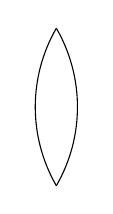
\begin{tikzpicture}
		%sets the lens shape
		\pgfmathsetmacro{\lensRadius}{2}
		\pgfmathsetmacro{\lensHeight}{1}
		\pgfmathsetmacro{\startAngle}{asin(\lensHeight/\lensRadius)}
		
		%draws the lens
		\draw (0,\lensHeight) arc[start angle=180-\startAngle,delta angle=2*\startAngle,radius=\lensRadius];
		\draw (0,\lensHeight) arc[start angle=\startAngle,delta angle=-2*\startAngle,radius=\lensRadius];
		
		%draws a dotted line through the middle of the lens
		%\draw[dash pattern=on5pt off3pt] (0,-1) -- (0,1) ;
		\end{tikzpicture}
				\caption{A Simple diagram representation of a convex lens}
	\end{center}
	\end{figure}



\item \textit{Concave} lenses, sometimes called \textit{diverging} lenses are larger at the edges than the center.  They are found in lenses for near-sightedness.  

\begin{center}
	\begin{figure}[H]
		\begin{center}

	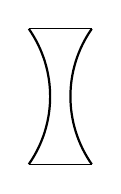
\begin{tikzpicture}
	

	
	\draw [thick, fill=white] (-.4,-.9) 	arc[start angle=-35, end angle=35,radius=1.5];
	\draw [thick, fill=white] (.4,-.9) 	arc[start angle=215, end angle=145,radius=1.5];
	
	\begin{scope}[>=latex]
	\draw [] (-.4,-.9) -- (.4,-.9);
	\draw [] (-.4,.82) -- (.4,.82);
	\end{scope}

		\end{tikzpicture}
				\caption{A Simple diagram representation of a concave lens}
				\end{center}
	\end{figure}
\end{center}

\end{itemize}


\paragraph{Convex Lenses} \index{Lens, Convex} \index{Convex Lens}



When parallel rays of light strike a convex lens, the light can be focused into a very small area.  The point at which the light is focused is called the \textit{focal point} \index{Focal Point.}  
\begin{center}
		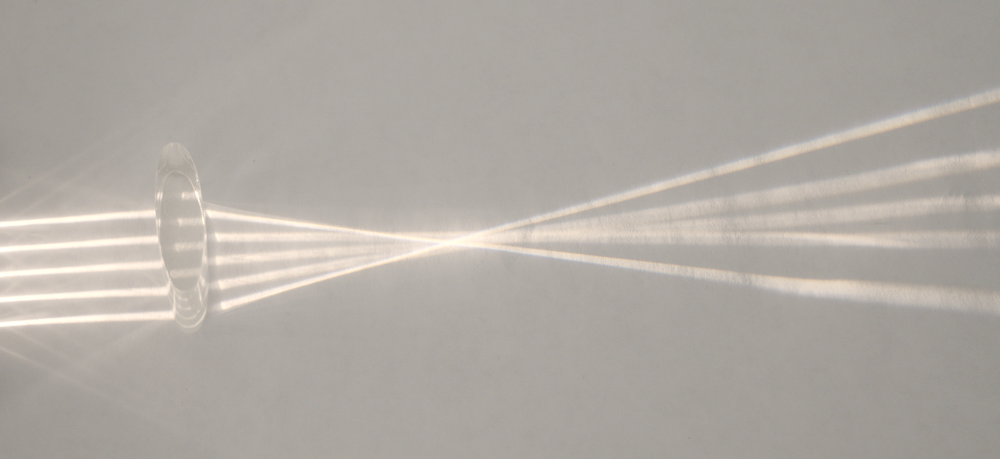
\includegraphics{./Chapters/Ch11-Optics/convex.png}
\end{center}

		
	\begin{figure} [H]
	
	\begin{center}
		\begin{tikzpicture}
		%sets the lens shape
		\pgfmathsetmacro{\lensRadius}{2}
		\pgfmathsetmacro{\lensHeight}{1}
		\pgfmathsetmacro{\startAngle}{asin(\lensHeight/\lensRadius)}
		
		%draws the lens
		\draw (0,\lensHeight) arc[start angle=180-\startAngle,delta angle=2*\startAngle,radius=\lensRadius];
		\draw (0,\lensHeight) arc[start angle=\startAngle,delta angle=-2*\startAngle,radius=\lensRadius];
		
		%draws a dotted line through the middle of the lens
		\draw[dash pattern=on5pt off3pt] (0,-1) -- (0,1) ;
		
		%incident Rays
		\draw[red,directed] (-5,.8) -- (0,.8) ;
		\draw[red,directed] (-5,.4) -- (0,.4) ;
		\draw[red,directed] (-5,.0) -- (0,.0) ;
		\draw[red,directed] (-5,-.4) -- (0,-.4) ;
		\draw[red,directed] (-5,-.8) -- (0,-.8) ;
		
		%Refracted rays
		\draw[red,directed] (0,.8) -- (5,-.8) ;
		\draw[red,directed] (0,.4) -- (5,-.4) ;
		\draw[red,directed] (0,.0) -- (5,.0) ;
		\draw[red,directed] (0,-.4) -- (5,.4) ;
		\draw[red,directed] (0,-.8) -- (5,.8) ;
		
		\node[below] at (2.5,0) {$f$};
		
		\end{tikzpicture}
		\caption{Light focused by a convex lens.  The focal point is labeled $f$.}
	\end{center}
\end{figure}




The distance from the center of the lens to the focal point is called the \textit{Focal Length.} \index{Focal Length}  Because light call pass through the lens either way, lenses have two focal points, both equidistant from the center of the lens.  

\subparagraph{Image Formation with Convex Lenses}
When a lens interacts with an object, an image is normally formed.  There are two often-used methods for determining where images form: \textit{Ray Tracing} and use of \textit{the lens equation.}

The method of ray tracing is performed in the following example: 

\begin{mdframed}[backgroundcolor=blue!10!white]
	\begin{center}	
		\textbf{Example \thesection.}	
	\end{center}
	
	\textbf{Problem:} A 1-cm tall object is placed 4 cm to the left of a lens of focal length $f=2 \si{cm}$.  Use ray-tracing to determine the position, size, and orientation of the image.  

\textbf{Solution}: 


\begin{enumerate}
	\item Begin by drawing a horizontal line across your paper.  This is your optical axis: 
	\vspace{.5 in}
	\begin{center}
		

	\begin{tikzpicture}
	%optical axis
	\draw (-7,0) -- (7,0);
	\end{tikzpicture}
		\end{center}
	\vspace{.5 in}
	
	
	
	\item Draw a lens on the optical axis.  Use a dotted line to represent the center of the lens.  
	

	\begin{center}
		
		
		\begin{tikzpicture}
		%draws the optical axis
		\draw (-7,0) -- (7,0);
		
			
		%sets the lens shape
		\pgfmathsetmacro{\lensRadius}{8}
		\pgfmathsetmacro{\lensHeight}{2}
		\pgfmathsetmacro{\startAngle}{asin(\lensHeight/\lensRadius)}
		
		%draws the lens
		\draw (0,\lensHeight) arc[start angle=180-\startAngle,delta angle=2*\startAngle,radius=\lensRadius];
		\draw (0,\lensHeight) arc[start angle=\startAngle,delta angle=-2*\startAngle,radius=\lensRadius];
		
		%draws a dotted line through the middle of the lens
		\draw[dash pattern=on5pt off3pt] (0,-2) -- (0,2) ;		
		\end{tikzpicture}
	\end{center}

	\item Measure and label focal points from the center of the lens, along the optical axis, and draw the object as an arrow with its base on the optical axis.
		\begin{center}
		
		
		\begin{tikzpicture}[place/.style={circle,fill=red}]
		%draws the optical axis
		\draw (-7,0) -- (7,0);
		
		
		%sets the lens shape
		\pgfmathsetmacro{\lensRadius}{8}
		\pgfmathsetmacro{\lensHeight}{2}
		\pgfmathsetmacro{\startAngle}{asin(\lensHeight/\lensRadius)}
		
		%draws the lens
		\draw (0,\lensHeight) arc[start angle=180-\startAngle,delta angle=2*\startAngle,radius=\lensRadius];
		\draw (0,\lensHeight) arc[start angle=\startAngle,delta angle=-2*\startAngle,radius=\lensRadius];
		
		%draws a dotted line through the middle of the lens
		\draw[dash pattern=on5pt off3pt] (0,-2) -- (0,2) ;	
		
		%draws focal points
		\node (n1) at (-2,0) [place] {};	
		\node (n21) at (2,0) [place] {};
		
			
		
		%draws object
		\draw [->,ultra thick] (-4,0) --(-4,1);
		\end{tikzpicture}
	\end{center}
	
\item The first ray of light will begin on the left of the diagram, graze the top of the object, and continue to the center of the lens.  It will then be directed down, through the far focal point.  

		\begin{center}
	
	
	\begin{tikzpicture}[place/.style={circle,fill=red}]
	%draws the optical axis
	\draw (-7,0) -- (7,0);
	
	
	%sets the lens shape
	\pgfmathsetmacro{\lensRadius}{8}
	\pgfmathsetmacro{\lensHeight}{2}
	\pgfmathsetmacro{\startAngle}{asin(\lensHeight/\lensRadius)}
	
	%draws the lens
	\draw (0,\lensHeight) arc[start angle=180-\startAngle,delta angle=2*\startAngle,radius=\lensRadius];
	\draw (0,\lensHeight) arc[start angle=\startAngle,delta angle=-2*\startAngle,radius=\lensRadius];
	
	%draws a dotted line through the middle of the lens
	\draw[dash pattern=on5pt off3pt] (0,-2) -- (0,2) ;	
	
	%draws focal points
	\node (n1) at (-2,0) [place] {};	
	\node (n21) at (2,0) [place] {};
	
	
	
	%draws object
	\draw [->, ultra thick] (-4,0) --(-4,1);
	
	
	%First Ray
	\draw [directed, ultra thick,red] (-7,1) --(0,1);
	\draw [directed, ultra thick,red] (0,1) --(6,-2);	
	\end{tikzpicture}
\end{center}

\item The second ray of light will graze the top of the object, pass through the near focal point, continuing until it hits the center of the lens.  There, the ray will be directed parallel to the optical axis.  

		\begin{center}
	
	
	\begin{tikzpicture}[place/.style={circle,fill=red}]
	%draws the optical axis
	\draw (-7,0) -- (7,0);
	
	
	%sets the lens shape
	\pgfmathsetmacro{\lensRadius}{8}
	\pgfmathsetmacro{\lensHeight}{2}
	\pgfmathsetmacro{\startAngle}{asin(\lensHeight/\lensRadius)}
	
	%draws the lens
	\draw (0,\lensHeight) arc[start angle=180-\startAngle,delta angle=2*\startAngle,radius=\lensRadius];
	\draw (0,\lensHeight) arc[start angle=\startAngle,delta angle=-2*\startAngle,radius=\lensRadius];
	
	%draws a dotted line through the middle of the lens
	\draw[dash pattern=on5pt off3pt] (0,-2) -- (0,2) ;	
	
	%draws focal points
	\node (n1) at (-2,0) [place] {};	
	\node (n21) at (2,0) [place] {};
	
	
	
	%draws object
	\draw [->, ultra thick] (-4,0) --(-4,1);
	
	
	%First Ray
	\draw [directed, ultra thick,red] (-7,1) --(0,1);
	\draw [directed, ultra thick,red] (0,1) --(6,-2);	
	
	%Second Ray
	\draw [directed, ultra thick,blue] (-6,2) --(0,-1);
	\draw [directed, ultra thick,blue] (0,-1) --(7,-1);	
	
	\end{tikzpicture}
\end{center}
	
	\item The final ray of light will graze the top of the object, directed toward the intersection of center of the lens and the optical axis.  This ray will not change direction.  The intersection of the three rays is where the top of the image will form.  
	
			\begin{center}
		
		
		\begin{tikzpicture}[place/.style={circle,fill=red}]
		%draws the optical axis
		\draw (-7,0) -- (7,0);
		
		
		%sets the lens shape
		\pgfmathsetmacro{\lensRadius}{8}
		\pgfmathsetmacro{\lensHeight}{2}
		\pgfmathsetmacro{\startAngle}{asin(\lensHeight/\lensRadius)}
		
		%draws the lens
		\draw (0,\lensHeight) arc[start angle=180-\startAngle,delta angle=2*\startAngle,radius=\lensRadius];
		\draw (0,\lensHeight) arc[start angle=\startAngle,delta angle=-2*\startAngle,radius=\lensRadius];
		
		%draws a dotted line through the middle of the lens
		\draw[dash pattern=on5pt off3pt] (0,-2) -- (0,2) ;	
		
		%draws focal points
		\node (n1) at (-2,0) [place] {};	
		\node (n21) at (2,0) [place] {};
		
		
		
		%draws object
		\draw [->, ultra thick] (-4,0) --(-4,1);
		
		
		%First Ray
		\draw [directed, ultra thick,red] (-7,1) --(0,1);
		\draw [directed, ultra thick,red] (0,1) --(6,-2);	
		
		%Second Ray
		\draw [directed, ultra thick,blue] (-6,2) --(0,-1);
		\draw [directed, ultra thick,blue] (0,-1) --(7,-1);	
		
		%Third Ray
		\draw [directed, ultra thick,green] (-6,1.5) --(0,0);
		\draw [directed, ultra thick,green] (0,0) --(6,-1.5);	
		
		\draw [->, ultra thick] (4,0) --(4,-1);
		
		
		\end{tikzpicture}
	\end{center}
	
	The diagram can then be measured.  In this case, the image is 4 cm to the right of the lens, inverted, and the same size as the object.  
	
\end{enumerate}


\end{mdframed}

The \textit{lens equation} \index{Lens Equation} can also be used to determine the distance to the image.  The lens equation is:

	\begin{mdframed}[backgroundcolor=orange!20!white]
	
	\begin{equation}
	\frac{1}{f} = \frac{1}{o} + \frac{1}{i}
	\label{equation:lens}
	\end{equation}
\end{mdframed}
 where $f$ is the focal length of the lens, $o$ is the object distance from the lens, and $i$ is the image distance from the lens.  
 
 The magnification of an image can be determined by the following equation:
 	\begin{mdframed}[backgroundcolor=orange!20!white]
 	
 	\begin{equation}
 	m = - \frac{i}{o} = \frac{h_i}{h_o}
 	\label{equation:magnification}
 	\end{equation}
 \end{mdframed}
 
 where $h_i$ is the image height, and $h_o$ is the object height.  
 
 
 
 \begin{mdframed}[backgroundcolor=blue!10!white]
 	\begin{center}	
 		\textbf{Example \thesection.5}	
 	\end{center}
 	
 	\textbf{Problem:} A 1-cm tall object is placed 4 cm to the left of a lens of focal length $f=2 \si{cm}$.  Use the lens equation and the magnification formula to determine the position, size, and orientation of the image.  
 	
 	\textbf{Solution}: In this case, we are given $h_o = 1 \si{cm}$, $o = 4 \si{cm}$ and $f = 2 \si{cm}$.  First, the lens equation is solved for $i$:
 	
 	\begin{equation*}
 	\frac{1}{f} = \frac{1}{o} + \frac{1}{i}  
 	\end{equation*}
 	
 	
 	\begin{equation*}
 	i = \frac{1}{\frac{1}{f}-\frac{1}{o}} = \frac{1}{\frac{1}{2\si{cm}}-\frac{1}{4\si{cm}}} = \boxed{4 \si{cm}}
 	\end{equation*}
 
 	
 	Calculating the magnification gives: 
 	
 	\begin{equation*}
 	m = - \frac{i}{o} = -\frac{4\si{cm}}{4\si{cm}} = \boxed{-1}
 	\end{equation*}
 	The negative magnification means that the image is inverted.  You may also notice that magnification is a unitless quantity.  Finally, calculating the height of the image shows that the image is the same size (thought inverted).  
 	
 	\begin{equation*}
 	m = \frac{h_i}{h_o} \longrightarrow h_i = m h_o = (-1)(1 \si{cm}) = \boxed{-1 \si{cm}}
 	\end{equation*}
 	
 	
 	
 \end{mdframed}
 


\newpage
\paragraph{Concave Lenses} \index{Lens, Concave} \index{Concave Lens}
Instead of being focused to a point, parallel rays of light that are incident upon a concave lens diverge, as shown below:

\begin{center}
	
		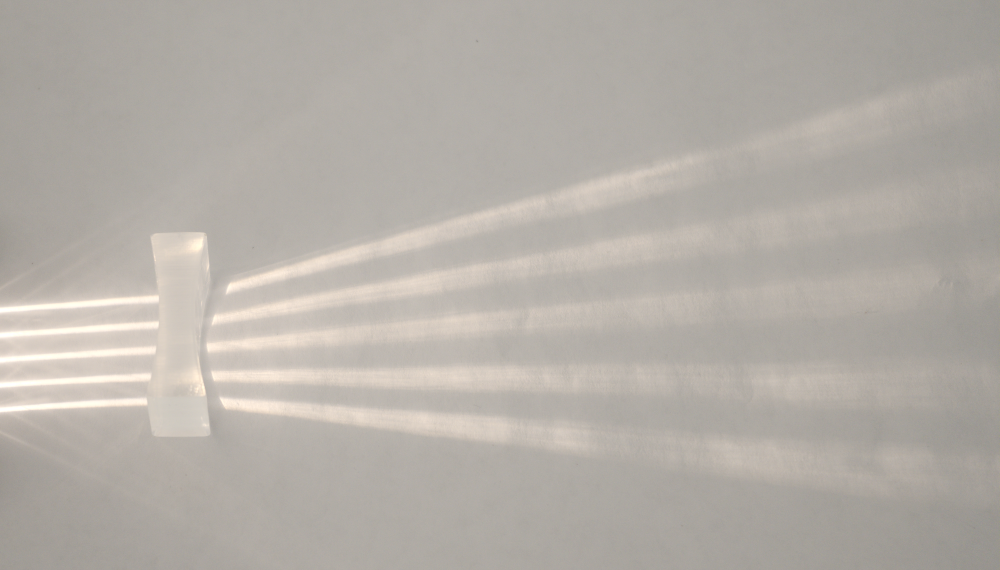
\includegraphics{./Chapters/Ch11-Optics/concave.png}
	
	
	
	\begin{figure}[H]
		\begin{center}
			
			\begin{tikzpicture}
				
				
				
				\draw [thick, fill=white] (-.4,-.9) 	arc[start angle=-35, end angle=35,radius=1.5];
				\draw [thick, fill=white] (.4,-.9) 	arc[start angle=215, end angle=145,radius=1.5];
				
				\begin{scope}[>=latex]
					\draw [] (-.4,-.9) -- (.4,-.9);
					\draw [] (-.4,.82) -- (.4,.82);
				\end{scope}
				
					%incident Rays
				\draw[red,directed] (-5,.6) -- (0,.6) ;
				\draw[red,directed] (-5,.3) -- (0,.3) ;
				\draw[red,directed] (-5,.0) -- (0,.0) ;
				\draw[red,directed] (-5,-.3) -- (0,-.3) ;
				\draw[red,directed] (-5,-.6) -- (0,-.6) ;
				%center line of lens
				
						\draw[dash pattern=on5pt off3pt] (0,-1) -- (0,1) ;
				
				%Refracted rays
				\draw[red,directed] (0,.6) -- (5,2) ;
				\draw[red,directed] (0,.3) -- (5,1) ;
				\draw[red,directed] (0,.0) -- (5,.0) ;
				\draw[red,directed] (0,-.3) -- (5,-1) ;
				\draw[red,directed] (0,-.6) -- (5,-2) ;
				
				
				
				
				
			\end{tikzpicture}
			\caption{A concave lens causes light rays to diverge.}
			\label{fig:concave}
		\end{center}
	\end{figure}
\end{center}

Though the rays do not converge on the right side of the lens in figure \ref{fig:concave}, the rays can be extended backward to show an apparent focal point on the wrong side of the lens:

\begin{center}
	\begin{figure}[H]
		\begin{center}
			
			\begin{tikzpicture}
			
			
			
			\draw [thick, fill=white] (-.4,-.9) 	arc[start angle=-35, end angle=35,radius=1.5];
			\draw [thick, fill=white] (.4,-.9) 	arc[start angle=215, end angle=145,radius=1.5];
			
			\begin{scope}[>=latex]
			\draw [] (-.4,-.9) -- (.4,-.9);
			\draw [] (-.4,.82) -- (.4,.82);
			\end{scope}
			
			%incident Rays
			\draw[red,directed] (-5,.6) -- (0,.6) ;
			\draw[red,directed] (-5,.3) -- (0,.3) ;
			\draw[red,directed] (-5,.0) -- (0,.0) ;
			\draw[red,directed] (-5,-.3) -- (0,-.3) ;
			\draw[red,directed] (-5,-.6) -- (0,-.6) ;
			%center line of lens
			
			\draw[dash pattern=on5pt off3pt] (0,-1) -- (0,1) ;
			
			%Refracted rays
			\draw[red,directed] (0,.6) -- (5,2) ;
			\draw[red,directed] (0,.3) -- (5,1) ;
			\draw[red,directed] (0,.0) -- (5,.0) ;
			\draw[red,directed] (0,-.3) -- (5,-1) ;
			\draw[red,directed] (0,-.6) -- (5,-2) ;
			
					
			\draw[dash pattern=on5pt off3pt,blue] (-5,-.8) -- (0,.6) ;
			\draw[dash pattern=on5pt off3pt,blue] (-5,.8) -- (0,-.6) ;			
			\draw[dash pattern=on5pt off3pt,blue] (-5,-.4) -- (0,.3) ;			
			\draw[dash pattern=on5pt off3pt,blue] (-5,.4) -- (0,-.3) ;	
			\draw[dash pattern=on5pt off3pt,blue] (-5,0) -- (0,0) ;	
			
			
			\end{tikzpicture}
			\caption{A concave lens appears to have a focal point on the other side of the lens.}
			\label{fig:concave2}
		\end{center}
	\end{figure}
\end{center}

Because concave lenses appear to have a focal point on the wrong side of the lens, their focal length is negative.  



\begin{mdframed}[backgroundcolor=blue!10!white]
	\begin{center}	
		\textbf{Example \thesection.6}	
	\end{center}
	
	\textbf{Problem:} A 1-cm tall object is placed 4 cm to the left of a lens of focal length $f=-2 \si{cm}$.  Use ray-tracing to determine the position, size, and orientation of the image.  
	
	\textbf{Solution}: 
	
	
	\begin{enumerate}
		\item Begin by drawing the optical axis and lens. Note that since the focal length is negative, this is a concave lens.   
		
		\begin{center}
			
			
			
\begin{tikzpicture}

			
					
			\draw [thick, fill=blue!10!white] (-.6,-2) 	arc[start angle=-30, end angle=30,radius=4];
			\draw [thick, fill=blue!10!white] (.6,-2) 	arc[start angle=210, end angle=150,radius=4];
			%draws the optical axis
			\draw (-7,0) -- (7,0);
			
			\begin{scope}[>=latex]
			\draw [] (-.6,-2) -- (.6,-2);
			\draw [] (-.6,2) -- (.6,2);
			\end{scope}
		
			
			%draws a dotted line through the middle of the lens
			\draw[dash pattern=on5pt off3pt] (0,-2) -- (0,2) ;		
			\end{tikzpicture}
		\end{center}
		
		\item Measure and label focal points from the center of the lens, along the optical axis, and draw the object as an arrow with its base on the optical axis.  Remember, that because the focal length is negative, the focal point for the right side is on the left, and the focal point for the left side is on the right.  
		\begin{center}
			
			
			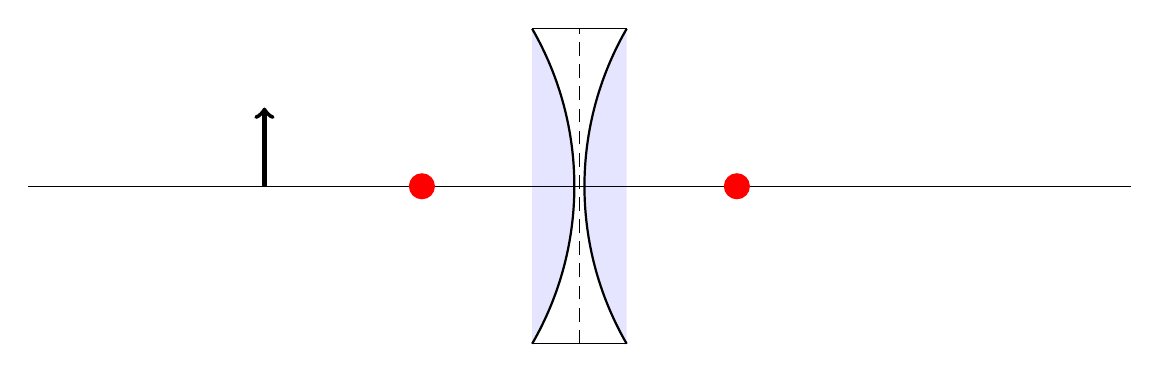
\begin{tikzpicture}[place/.style={circle,fill=red}]
			%draws the optical axis
			
	\draw [thick, fill=blue!10!white] (-.6,-2) 	arc[start angle=-30, end angle=30,radius=4];
	\draw [thick, fill=blue!10!white] (.6,-2) 	arc[start angle=210, end angle=150,radius=4];
	%draws the optical axis
	\draw (-7,0) -- (7,0);
	
	\begin{scope}[>=latex]
	\draw [] (-.6,-2) -- (.6,-2);
	\draw [] (-.6,2) -- (.6,2);
	\end{scope}


	%draws a dotted line through the middle of the lens
	\draw[dash pattern=on5pt off3pt] (0,-2) -- (0,2) ;		
			\draw[dash pattern=on5pt off3pt] (0,-2) -- (0,2) ;	
			
			%draws focal points
			\node (n1) at (-2,0) [place] {};	
			\node (n21) at (2,0) [place] {};
			
			
			
			%draws object
			\draw [->,ultra thick] (-4,0) --(-4,1);
			\end{tikzpicture}
		\end{center}
		
		\item The first ray of light will begin on the left of the diagram, graze the top of the object, and continue to the center of the lens.  It will then be directed upward, as if it came from the right focal point (which is actually on the left).  
		
		\begin{center}
			
			
			\begin{tikzpicture}[place/.style={circle,fill=red}]
			%draws the optical axis

		\draw [thick, fill=blue!10!white] (-.6,-2) 	arc[start angle=-30, end angle=30,radius=4];
		\draw [thick, fill=blue!10!white] (.6,-2) 	arc[start angle=210, end angle=150,radius=4];
		%draws the optical axis
		\draw (-7,0) -- (7,0);
		
		\begin{scope}[>=latex]
		\draw [] (-.6,-2) -- (.6,-2);
		\draw [] (-.6,2) -- (.6,2);
		\end{scope}


	%draws a dotted line through the middle of the lens
	\draw[dash pattern=on5pt off3pt] (0,-2) -- (0,2) ;		
	\draw[dash pattern=on5pt off3pt] (0,-2) -- (0,2) ;	

	%draws focal points
	\node (n1) at (-2,0) [place] {};	
	\node (n21) at (2,0) [place] {};



	%draws object
	\draw [->,ultra thick] (-4,0) --(-4,1);
			
			
			%First Ray
			\draw [directed, ultra thick,red] (-7,1) --(0,1);
			\draw[dash pattern=on5pt off3pt,red] (-4,-1) -- (0,1) ;	
			\draw [directed, ultra thick,red] (0,1) --(4,3);	
			\end{tikzpicture}
		\end{center}
		
		\item The second ray of light will graze the top of the object and be directed toward the near focal point (which is on the far side of the lens).  Upon encountering the optical axis, the ray will be directed parallel to the optical axis.  
		
		\begin{center}
			
			
			\begin{tikzpicture}[place/.style={circle,fill=red}]
					%draws the optical axis
		
		\draw [thick, fill=blue!10!white] (-.6,-2) 	arc[start angle=-30, end angle=30,radius=4];
		\draw [thick, fill=blue!10!white] (.6,-2) 	arc[start angle=210, end angle=150,radius=4];
		%draws the optical axis
		\draw (-7,0) -- (7,0);
		
		\begin{scope}[>=latex]
		\draw [] (-.6,-2) -- (.6,-2);
		\draw [] (-.6,2) -- (.6,2);
		\end{scope}
		
		
		%draws a dotted line through the middle of the lens
		\draw[dash pattern=on5pt off3pt] (0,-2) -- (0,2) ;		
		\draw[dash pattern=on5pt off3pt] (0,-2) -- (0,2) ;	
		
		%draws focal points
		\node (n1) at (-2,0) [place] {};	
		\node (n21) at (2,0) [place] {};
		
		
		
		%draws object
		\draw [->,ultra thick] (-4,0) --(-4,1);
		
		
		%First Ray
		\draw [directed, ultra thick,red] (-7,1) --(0,1);
		\draw[dash pattern=on5pt off3pt,red] (-4,-1) -- (0,1) ;	
		\draw [directed, ultra thick,red] (0,1) --(4,3);
			
			%Second Ray
			\draw [directed, ultra thick,blue] (-6,1.333) --(0,.333);
			\draw [directed, ultra thick,blue] (0,.333) --(7,.333);	
			\draw[dash pattern=on5pt off3pt,blue] (-7,.3333) -- (0,.3333) ;				
			\draw[dash pattern=on1pt off1pt,black] (0,.3333) -- (2,0) ;			
			\end{tikzpicture}
		\end{center}
		
		\item The final ray of light will graze the top of the object, directed toward the intersection of center of the lens and the optical axis.  This ray will not change direction.  The intersection of the three rays is where the top of the image will form.  
		
		\begin{center}
			
			
			\begin{tikzpicture}[place/.style={circle,fill=red}]
								%draws the optical axis
			
			\draw [thick, fill=blue!10!white] (-.6,-2) 	arc[start angle=-30, end angle=30,radius=4];
			\draw [thick, fill=blue!10!white] (.6,-2) 	arc[start angle=210, end angle=150,radius=4];
			%draws the optical axis
			\draw (-7,0) -- (7,0);
			
			\begin{scope}[>=latex]
			\draw [] (-.6,-2) -- (.6,-2);
			\draw [] (-.6,2) -- (.6,2);
			\end{scope}
			
			
			%draws a dotted line through the middle of the lens
			\draw[dash pattern=on5pt off3pt] (0,-2) -- (0,2) ;		
			\draw[dash pattern=on5pt off3pt] (0,-2) -- (0,2) ;	
			
			%draws focal points
			\node (n1) at (-2,0) [place] {};	
			\node (n21) at (2,0) [place] {};
			
			
			
			%draws object
			\draw [->,ultra thick] (-4,0) --(-4,1);
			
			
			%First Ray
			\draw [directed, ultra thick,red] (-7,1) --(0,1);
			\draw[dash pattern=on5pt off3pt,red] (-4,-1) -- (0,1) ;	
			\draw [directed, ultra thick,red] (0,1) --(4,3);
			
			%Second Ray
			\draw [directed, ultra thick,blue] (-6,1.333) --(0,.333);
			\draw [directed, ultra thick,blue] (0,.333) --(7,.333);	
			\draw[dash pattern=on5pt off3pt,blue] (-7,.3333) -- (0,.3333) ;				
			\draw[dash pattern=on1pt off1pt,black] (0,.3333) -- (2,0) ;	
			
			%Third Ray
			\draw [directed, ultra thick,green] (-6,1.5) --(0,0);
			\draw [directed, ultra thick,green] (0,0) --(6,-1.5);	
			
			\draw [->, ultra thick,dash pattern=on1pt off1pt,black] (-1.333,0) --(-1.333,.333);
			
			
			\end{tikzpicture}
		\end{center}
		
		In this case, the image is behind the lens, meaning it is virtual.  It is upright, and smaller than the original.  Measuring the image distance yields $i=-1.333\si{cm}$ (that is, the image is 1.333 cm to the left of the lens).
		
		 
		
	\end{enumerate}
	
	
\end{mdframed}


The same problem can be solved using the lens equation as well:

 \begin{mdframed}[backgroundcolor=blue!10!white]
	\begin{center}	
		\textbf{Example \thesection.5}	
	\end{center}
	
	\textbf{Problem:} A 1-cm tall object is placed 4 cm to the left of a lens of focal length $f=-2 \si{cm}$.  Use the lens equation and the magnification formula to determine the position, size, and orientation of the image.  
	
	\textbf{Solution}: In this case, we are given $h_o = 1 \si{cm}$, $o = 4 \si{cm}$ and $f = -2 \si{cm}$.  First, the lens equation is solved for $i$:
	
	\begin{equation*}
	\frac{1}{f} = \frac{1}{o} + \frac{1}{i}  
	\end{equation*}
	
	
	\begin{equation*}
	i = \frac{1}{\frac{1}{f}-\frac{1}{o}} = \frac{1}{\frac{1}{-2\si{cm}}-\frac{1}{4\si{cm}}} = \boxed{-\frac{4}{3} \si{cm} \approx -1.333 \si{cm}}
	\end{equation*}
	
	
	Calculating the magnification gives: 
	
	\begin{equation*}
	m = - \frac{i}{o} = -\frac{-\frac{4}{3}\si{cm}}{4\si{cm}} = \boxed{\frac{1}{3}}
	\end{equation*}
	The positive magnification means that the image is inverted.  Since the magnification of this image is less than one, the image will appear smaller.  Finally, we calculate image height:  
	
	\begin{equation*}
	m = \frac{h_i}{h_o} \longrightarrow h_i = m h_o = (\frac{1}{3}) (1 \si{cm}) = \boxed{\frac{1}{3} \si{cm}}
	\end{equation*}
\end{mdframed}





		

	\subsection{Reflection} \index{Reflection}
	
			\subsubsection{The Law of Reflection} \index{Reflection, Law of} \index{Law of Reflection} 
			Compared to refraction, the law of reflection is quite simple: the angle of incidence is equal to the angle of reflection.  
			
			
					\begin{figure}[H]
				
				
				\begin{center}
					
					
					\begin{tikzpicture}[thick,scale=0.5, every node/.style={scale=0.5}]
					
					% define coordinates
					\coordinate (O) at (0,0) ;
					\coordinate (A) at (0,4) ;
					\coordinate (B) at (0,-.2) ;
					
					% media
					\fill[blue!15!,opacity=.3] (-4,0) rectangle (4,4);
					\fill[gray!60!,opacity=.9] (-4,0) rectangle (4,-.2);

					\node[right] at (4,-0.1) {Mirror};
		
					
					
					% axis
					\draw[dash pattern=on5pt off3pt] (A) -- (B) ;
					
					
					% rays
					\draw[red,ultra thick,reverse directed] (O) -- (130:5.2);
					\draw[red,directed,ultra thick] (O) -- (50:5.2);
					
					% angles
					\draw (0,1) arc (90:130:1);
					\draw (0,1) arc (90:50:1) ;
					\node[] at (70:1.4)  {$\theta_{r}$};
					\node[] at (110:1.4)  {$\theta_{i}$};
					
					\end{tikzpicture}
					\caption{The angle of incidence is equal to the angle of reflection}
				\end{center}
			\end{figure}
			
			This law of reflection can be expressed as the following equation.
			
			
		\begin{mdframed}[backgroundcolor=orange!20!white]		
			\begin{equation}
			\theta_{i} = \theta_{r}
			\label{eqn:lawofreflection}
			\end{equation}
	\end{mdframed}	
						
			
		\subsubsection{Mirrors} \index{Mirrors}		
		\paragraph{Flat Mirrors} \index{Mirrors, Flat}
		Flat mirrors are quite easy to work with.  The images produced by a flat mirror are always virtual, always the same size as the original object, and always upright.  For this reason, flat mirrors are often used in bathrooms and fitting rooms to give an accurate assessment of one's appearance.  		
		\paragraph{Concave Mirrors} \index{Mirrors, Concave}
		
		
				
		\paragraph{Convex Mirrors} \index{Mirrors, Convex}
		
		
	\section{Physical Optics}
		\subsection{Diffraction}
		\subsection{Young's Double Slit Experiment}
		\subsection{Thin Film Interference}
		
		
		
	

	


